

While deep learning has enabled highly performative modeling for various computer vision tasks~\cite{sota_imclass, sota_objdet}, large quantities of annotated data are still required for achieving \textit{state-of-the-art} performance~\cite{alex2019big}. This predicament is further exacerbated for tasks such as semantic segmentation, where the dense pixel-level annotations required for training can be prohibitively expensive. Various semi-supervised~\cite{semi_aug_2, domain_seg_nips_2, semi_sup_seg_1}, and self-supervised methods~\cite{self_sup_aaai, self_sup_iccv} have been proposed to alleviate this data-bottleneck, however they bring their own set of challenges such as domain-shift.

While dense annotation is costly~\cite{benenson2019large,kuznetsova2018open,cs_dataset}, collecting raw sequential image data is relatively cheap. This is especially the conventional methodology for autonomous driving datasets, such as~\cite{cs_dataset, as_dataset, argo_dataset}. Such datasets are often sparsely annotated across time (for example, in~\cite{cs_dataset}, pixel-level segmentation is provided once in every continuous partition of 30 frames). To assuage the data bottleneck, we can generate approximated labels for the unlabelled samples. 
While weak labels can be generated via \textit{lazy labelling}~\cite{lazy_label}, or pseudo-semantic annotations~\cite{taskonomy2018,pseudo_nips_1}, 
 the presence of an annotated sample in a continuous temporal sequence motivates the use of label propagation~\cite{lp_2006, lp_2010} for generating the approximated labels of neighbouring frames. 
 
\let\clearpage\relax
	\begin{figure}[t]
		\label{fig:comparison}
		\centering
		\subfigure[We propose a novel approach for propagation as well as training.]
		{
			\begin{minipage}{0.65\textwidth}
				\centering
				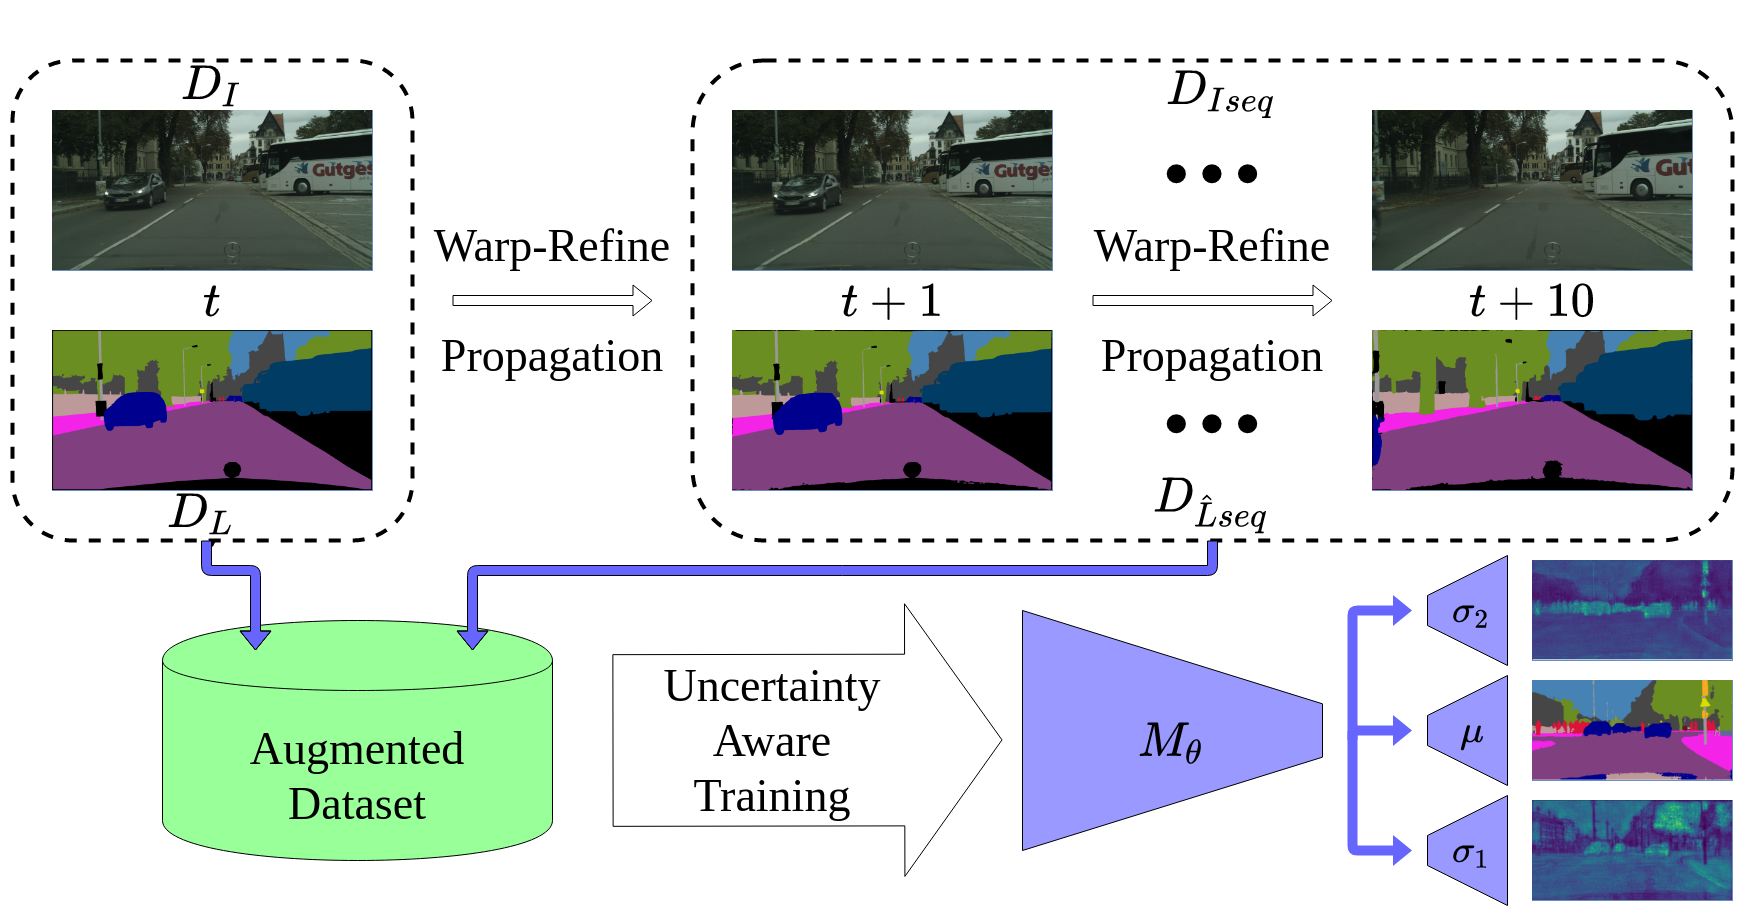
\includegraphics[width=1.0\linewidth]{figures/overview_lr.png}
				\vfill
			\end{minipage}
		}
		\hfill
        \hspace{-2em}
		\subfigure[Top:~\cite{nvidia_cvpr19}, Bottom: Ours]
		{
            % \begin{minipage}[b][0.315\textheight][s]{0.315\textwidth}
            \begin{minipage}{0.33\textwidth}
% \subfloat[(a)]{%
%   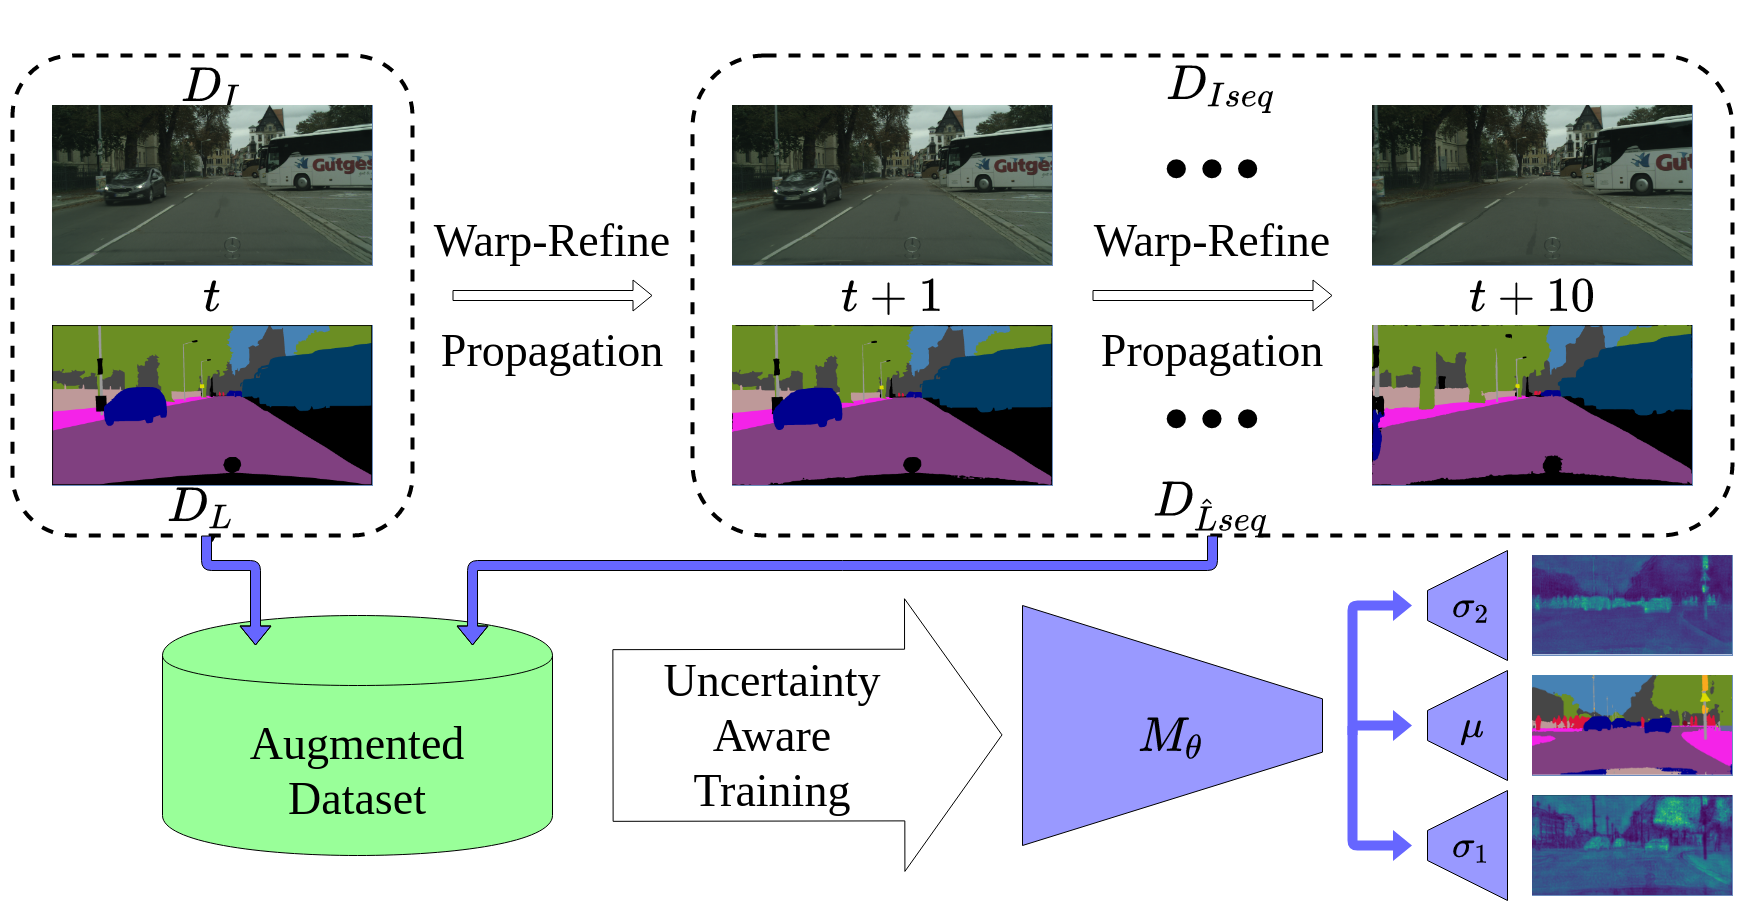
\includegraphics[clip,width=0.315\textwidth]{figures/fig_overview_lowres.png}%
% }
% \subfloat[(b)]{%
%   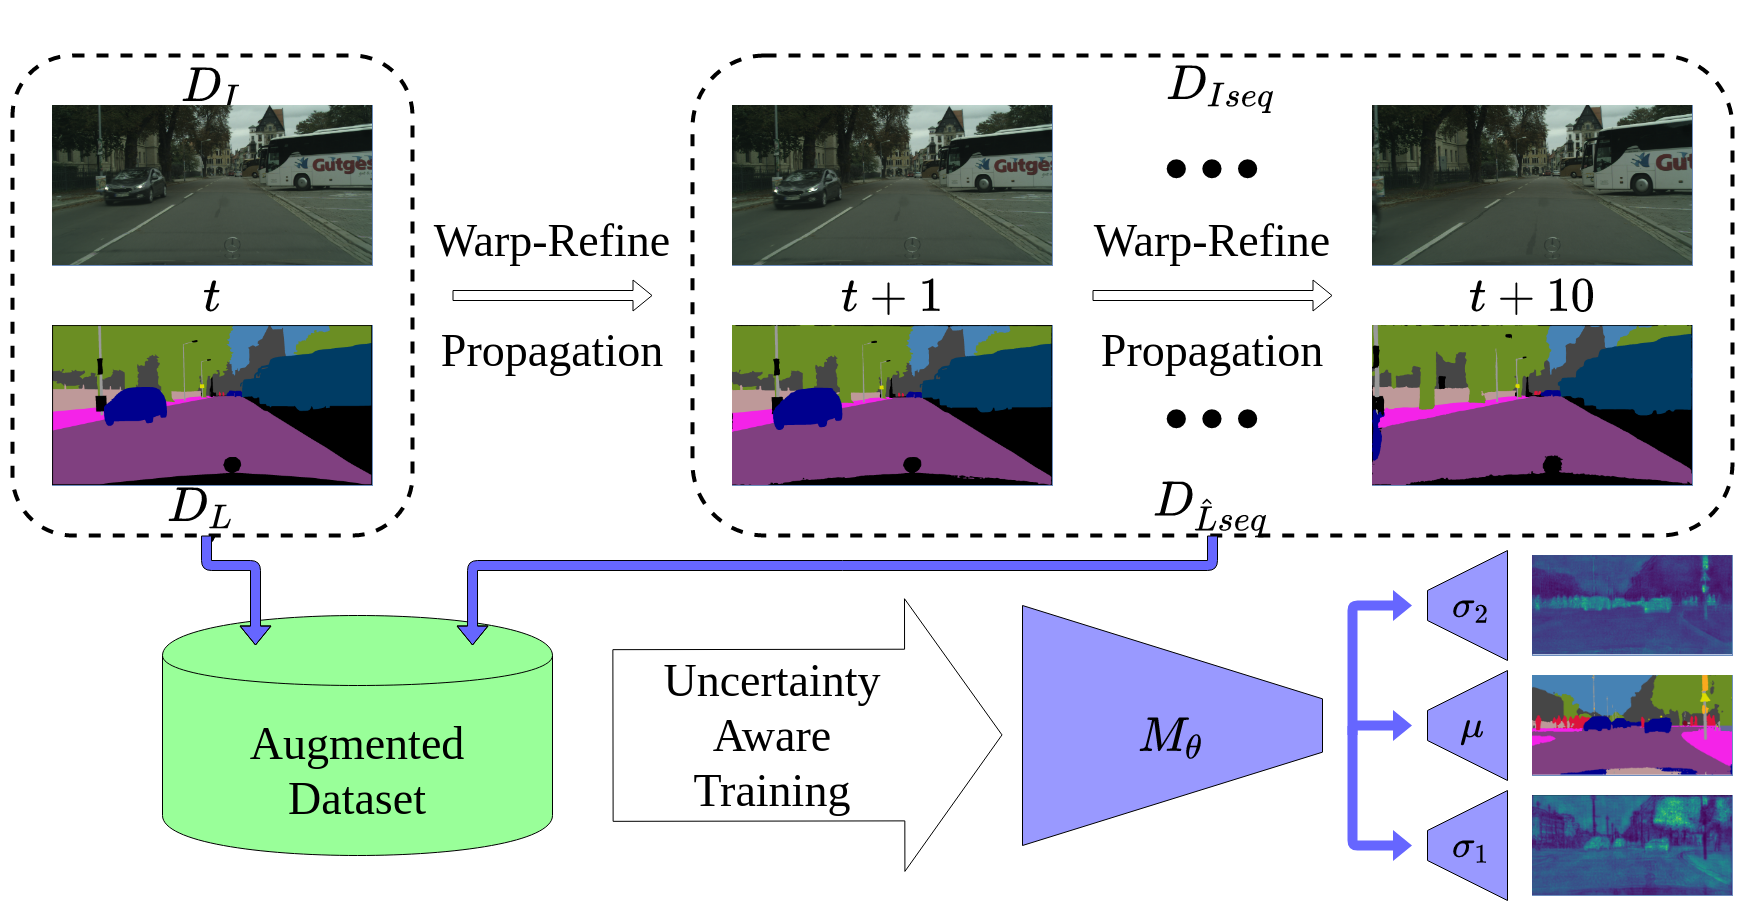
\includegraphics[clip,width=0.315\textwidth]{figures/fig_overview_lowres.png}%
% }
				\centering
				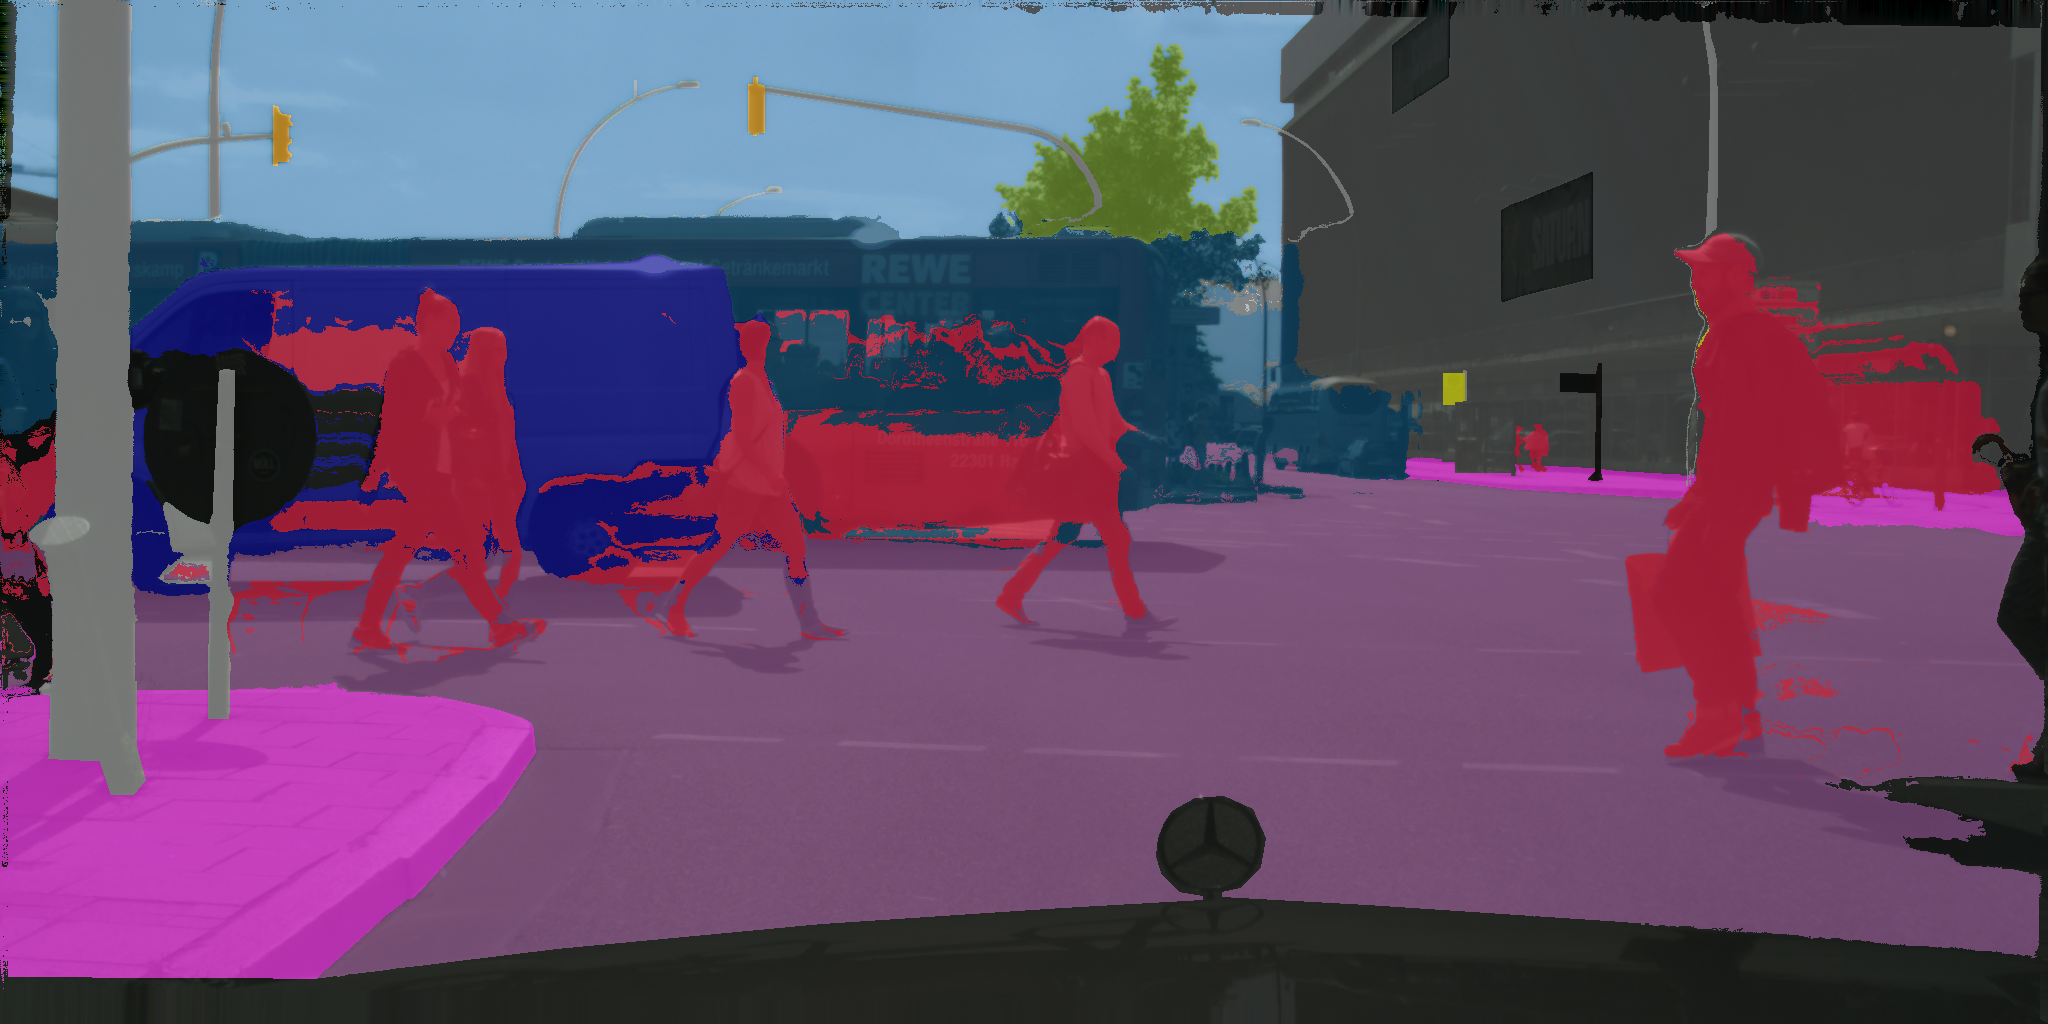
\includegraphics[width=\textwidth]{figures/prev_2.png}
				\vfill
				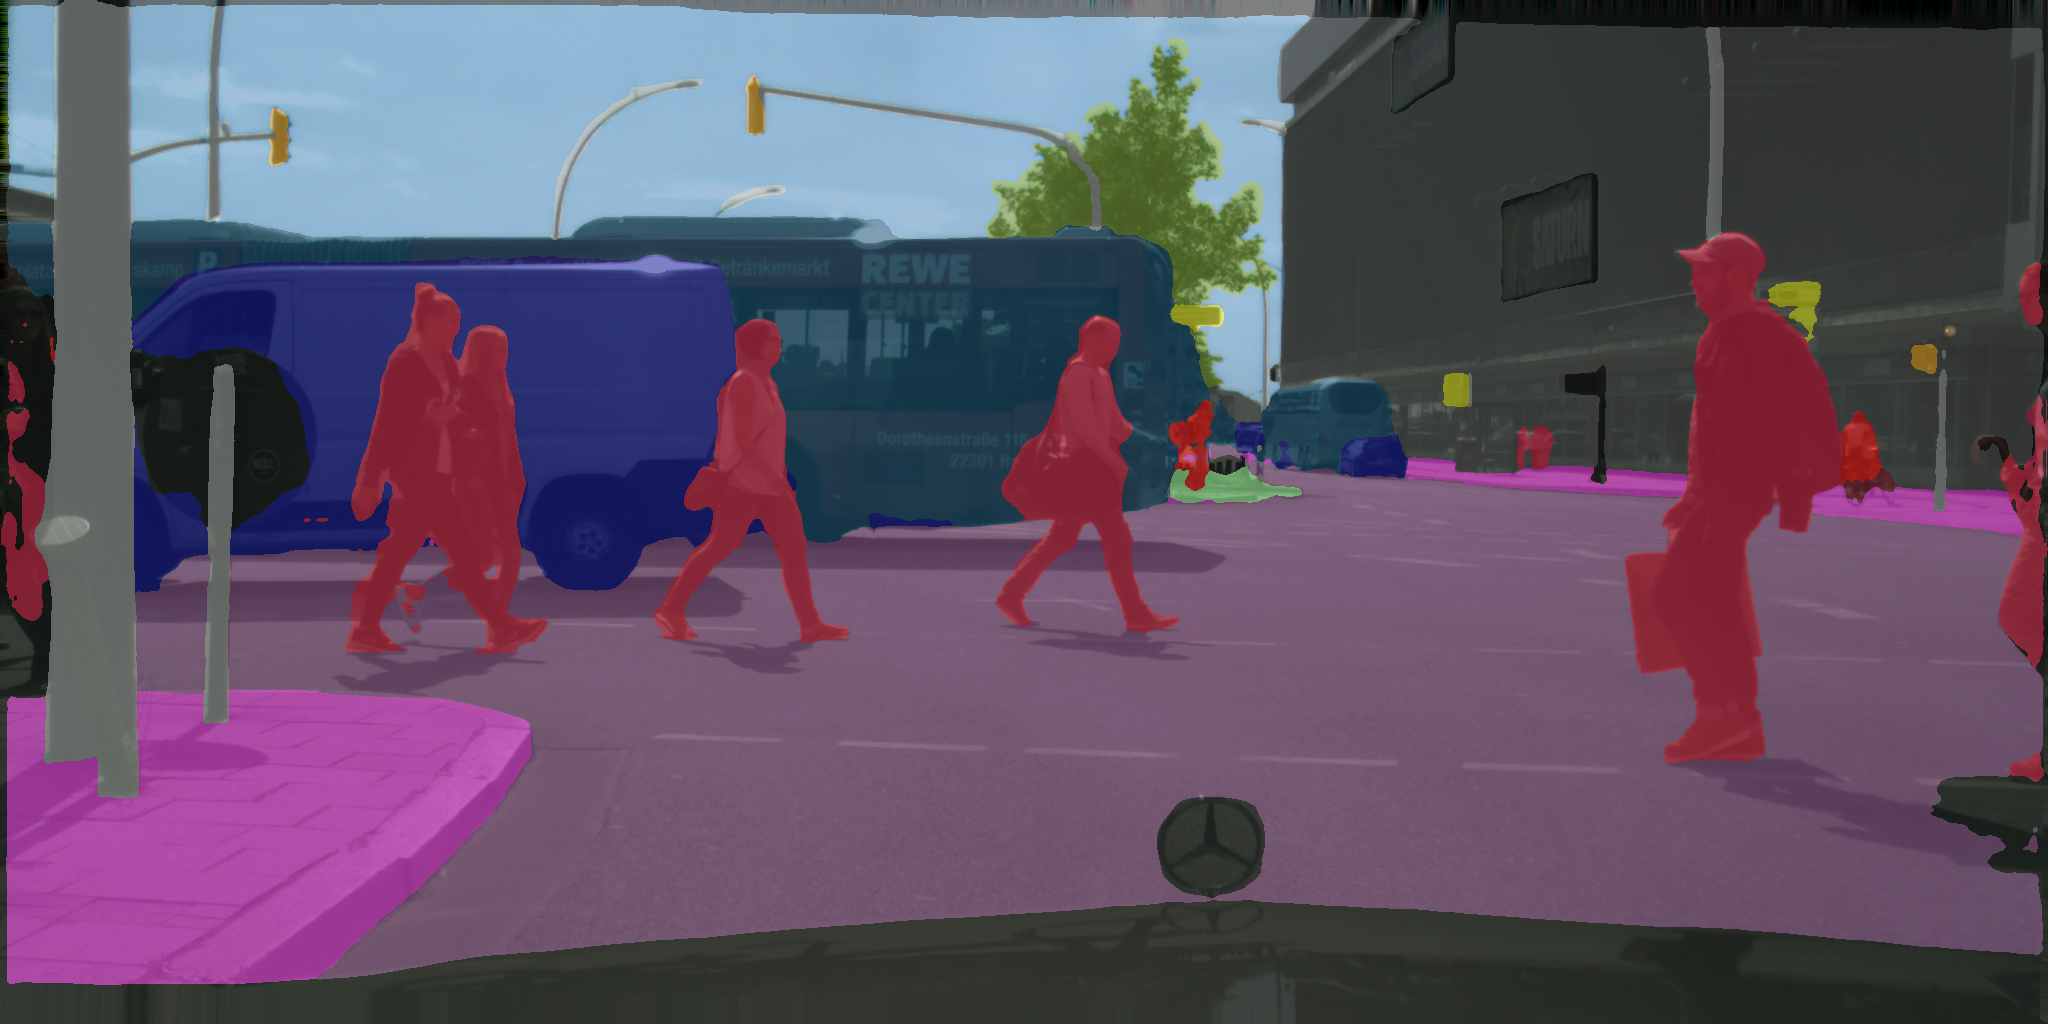
\includegraphics[width=\textwidth]{figures/our_2.png}%
				\vspace{0.3em}
			\end{minipage}
		}
    \vspace{-0.5em}
		\caption{\small (a) Using our propagation method, we generate pseudo-labels for images $D_{Iseq}$. The generated and the clean labels are then used for uncertainty-aware-training of semantic segmentation models. (b) Our method significantly surpasses \textit{state-of-the-art} label propagation methods~\cite{nvidia_cvpr19}.
		}
		\vspace{-0.5em}
	\end{figure}


The two primary concerns regarding label propagation are: a) \textit{How to perform it?} and b) \textit{How to utilize the generated labels?} In this work, we address both: We propose a new method to improve label propagation, and a principled approach for training with generated noisy labels. 

% The current \textit{state-of-the-art} method [], utilizes a \textit{video-reconstruction} model for label propagation. 
% The model, given the labelled image and its adjacent image, estimates a warping function from the labelled image to the adjacent image. The same estimated warping function, which is in the form of pixel-level motion vectors, is then applied to the labels to yield \textit{pseudo-labels} for the adjacent image. 
% By employing this model recurrently on a image sequence, the authors propagate labels to images further apart from the labelled image. However, 
Previous methods~\cite{lp_iccvw, lp_eccv, nvidia_cvpr19}, due to their reliance on geometric cues, have several of the same drawbacks as that of optical flow estimation. Specifically, prominent features of real-world data such as the lack of brightness consistency, or large motions, introduce harmful noise in the propagated labels. This drawback is further aggravated by the accumulation of errors as labels are propagated further in time. This is crucial, as longer propagation can yield more diverse labelled data, which is more beneficial for training deep neural networks~\cite{lp_eccv}.

Specifically, we make two important observations w.r.t previous propagation methods~\cite{lp_eccv, nvidia_cvpr19}: 1) They do not leverage the semantic knowledge in the annotated dataset, and 2) The noise in labels propagated with geometric methods has a systemic component which can be modelled. We propose a new propagation method called \emph{Warp-Refine Propagation} addressing both of these concerns. This method consists of two steps, a label warping step followed by a label refinement step. At the heart of our approach is the concept of cyclic consistency of labels, which we explain in detail in Section~\ref{subsec-alea}. As shown in Figure~\ref{fig:comparison}, our method significantly outperforms previous methods. 

In spite of the improvements, the propagated labels can still be noisy, especially when propagation takes place for larger time steps. 
% This is problematic as deep network can memorize noise in labels, leading to poor generalization~\cite{noisy_memory}.
% Furthermore, the noise does not allow us to use propagated labels which are further away, and contain more novel information. 
To address this challenge, we formulate \emph{Uncertainty-Aware Training}, a principled approach for training with noisy labels which contrasts previous heuristic methods such as label relaxation~\cite{nvidia_cvpr19} or loss weighting~\cite{lp_eccv}. 
We train the model to estimate the probability of the noisy labels under the true label distribution. This allows us to estimate the uncertainty of each label generation process, mitigating the drawbacks of training with noisy labels.
% Further, we provide theoretical proof that our approach implicitly reduces the total variational distance between the model and the true underlying distribution.
% In brief, we model the relation between noisy labels and the true labels in the form of label uncertainty, which alleviates the drawbacks of training with noisy labels. 
Furthermore, our approach can be used for multiple noisy distributions at the same time. Hence, with minimal changes to our model, we are also able to use pseudo-labelling~\cite{taskonomy2018,pseudo_nips_1}, i.e. noisy predictions from a pretrained-model, for data points where propagation is not possible. 
%In section~\ref{subsec-alea}, we draw the link between our approach and modelling of aleatoric uncertainty~\cite{gal_main} for different data generation processes. 

By using our propagation method, and our noisy label learning approach, we are able to achieve \textit{state-of-the-art} performance for two large scale autonomous driving datasets, namely Cityscapes, and ApolloScape. Further, we provide quantitative evaluation of various propagation methods which has crucially been missing from previous literature.

In summary, we 
\begin{itemize}
    \item Improve label propagation with a new approach called \emph{Warp-Refine Propagation}, and provide quantitative as well as qualitative evaluation for the same. 
    \item Propose \emph{Uncertainty-Aware Training}, a principled approach for learning with noisy labels, for which we further provide theoretical justification.
    \item Utilize our proposed advancements to achieve \textit{state-of-the-art} performance for two real-world autonomous driving datasets.
\end{itemize}



% TO BE SHORTENED.